\documentclass[12pt,UTF8,a4]{article}
\usepackage{amsmath, amssymb}
\usepackage{indentfirst}
\usepackage{multirow}
\usepackage{titlesec}
\usepackage{graphicx}
\usepackage{longtable}
\usepackage{framed}
\usepackage[noend]{algorithmic}
\usepackage{algorithm}
\usepackage{sectsty}
\usepackage{setspace}
\usepackage[footnotesize]{caption}
\usepackage{enumitem}
\usepackage[text={18cm,24cm}]{geometry}
\usepackage[hyperfigures,bookmarksnumbered,bookmarksopen,bookmarks,colorlinks,citecolor=blue,linkcolor=blue]{hyperref}
\usepackage{natbib}
\usepackage{mathpartir}

\setlength{\bibsep}{0.0pt}
\algsetup{indent=2em}
\setlength{\parindent}{2em} \setlength{\parskip}{3pt plus1pt minus1pt}

\DeclareGraphicsExtensions{.pdf,.png,.jpg}

\newcommand{\code}[1]{\texttt{#1}}
\newcommand{\type}[1]{\texttt{#1}}


\sectionfont{\large}
\subsectionfont{\normalsize}
\paragraphfont{\small}

\singlespacing
\title{CSCE 604 Final Project Report \\ Design and Implementation of a 2D Programming Language}
\author{Robert Schumacher, Plamen Ivanov and Peihong Guo}
\date{\today}

\begin{document}
\maketitle
\singlespacing

\section{Introduction}
We designed and implemented a two dimensional programming language featuring an interactive graphical programming environment in this project.

\section{Design Decisions}
\subsection{Language Specification}
====================================
\subsubsection{Visual Grammar}
The main element of the visual grammar will be called a "component". Each component will be described by a type signature. For example, an if-then-else component may be given the following type signature:
 if-then-else::Boolean->Integer. Components will be composed of an input, output, a name (if applicable) and a body.
 An input (or output) can be a tuple of any size composed of valid data types. An output from one component will serve as a feed for the 
input of another. Input and Outputs of different type will not be compatible allowing for a way for components to be strung together correctly.
 The body of a component can be composed of any number of other components, as long as they are connected correctly and provide an output for 
the containing component. Using such components, the programmer will be able to visually construct a program. The resulting structure of connected components will have the form of a graph. The graph will represent the structure of the program much better than sequentially written code.
 Places for parallelizing will be apparent from simply viewing the graph. Components will form nodes in the graph and connections between output and input will form edges. The graph will also have a recursive structure as individual nodes can be composed of large graphs themselves.

This visual language will need to be pure. This is necessary since, there are no guarantees for the sequence of execution of some possible programs. If side effects are allowed, it will be very difficult to keep track of them or debug the resulting programs.

The following figure is an example of how we envision the graphical language will look like:

This figure demonstrates the input/output matching and the definition of a function SUM-TUPLE, which takes a tuple of two Integers and returns their sum.

Translation:

The visual language above will have to be translated to a regular language. The main step for doing this will be to serialize the graph formed 
by the visual language. We can do that by using a topological sorting of the nodes in the graph. It has to be noted that topological sorting can result
 in many valid sorts. Additional rules may be needed to ensure an efficient translation.


Regular Grammar:

The visual language will be translated into a regular language. We can use a basic language which  supports a few data types, such as Integers, Boolean, String and Tuples. Some of the details of the language to translate into are still in the process of development.

====================================

\subsection{Basic Framework}
\subsubsection{Structure of Programs}
A program in the 2D programming language is a collection of definitions. A definition is the basic building block, which may contain predefined definitions, special definitions and user defined definitions.

Special definitions include \code{input}, \code{output}, \code{if}, \code{constant} and \code{arithmetic}.
\begin{table}[h]
\center
\begin{tabular}{c|c}
\hline
name & usage \\
\hline
\code{input} & defines input for a definition\\
\code{output} & the output of a definition\\
\code{if} & definition of \code{if} expression control flow \\
\code{constant} & definition of constants \\
\code{arithmetic} & definition of arithmetic expressions \\
\code{recursion} & definition of recursion\\
\hline
\end{tabular}
\caption{Special items.}\label{tab:sitems}
\end{table}

Predefined definitions include \code{print}, \code{pair}, \code{fst}, \code{snd}, \code{StringOfNumber}, \code{StringOfBool}, \code{Single}, \code{Nil}, \code{Head}, \code{Tail}, \code{Length}, \code{Append} and \code{Concat}.
\begin{table}[h]
\center
\begin{tabular}{c|c}
\hline
name & usage \\
\hline
\code{print} & print the content passed to its input node\\
\code{pair} & make a pair out of its two inputs\\
\code{fst} & break a pair and take its first item \\
\code{snd} & break a pair and take its second item \\
\code{StringOfNumber} & convert a number into a string\\
\code{StringOfBool} & convert a boolean value into a string \\
\code{Single} & \\
\code{Nil} & \\
\code{Head} & \\
\code{Tail} & \\
\code{Length} & \\
\code{Append} & \\
\code{Concat} & \\
\hline
\end{tabular}
\caption{Predefined items.}\label{tab:pitems}
\end{table}

The system maintains a global list of definitions, including predefined ones and special ones. Each definition in the list has a unique id, which is used as identifiers where they are referenced. These definitions are referenced wherever used, such as inside the body of a specific definition. For special definitions, new instances of them will be created whenever they are added to a user-defined definition. Predefined definitions are treated in the same way as special definitions to simplify the implementation, though they behave exactly the same as user-defined definitions.

\subsubsection{Structure of Definition}
Each definition consists of input, output, and a definition body. The body of a definition may include other definitions, such as predefined definitions or user-defined definitions.

The input of a definition can be empty, which corresponds to a definition that does not require an input. Definitions of this type are \code{input}, \code{constant}.

The body of a definition is a set of nodes referring to definitions. The member nodes of a definition are connected by a set of edges indicating the input-output dependencies between nodes, as is shown in Figure~\ref{fig:defbody}.

\begin{figure}[h]
\center
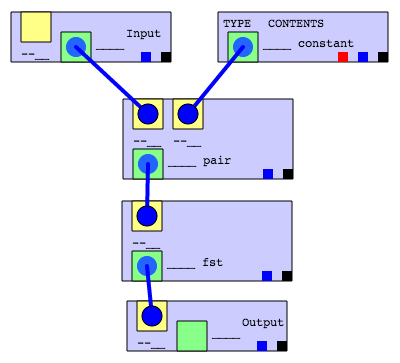
\includegraphics[width=0.5\textwidth]{./images/defbody}
\caption{The body of a definition for \code{identity} function.}\label{fig:defbody}
\end{figure}

Note the input and output nodes in Figure~\ref{fig:defbody} determines the input this definition is taking and the output of this definitions. A single input node indicates this definition, which is essentially an identity function, takes only one input. If multiple input nodes are included in the definition body, the function being defined takes a number of inputs.

A node in the body of a definition can be a reference to a user-defined definition, as is shown in Figure~\ref{fig:ref}. Here the \code{identity} node is a reference to the function defined in Figure~\ref{fig:defbody}.
\begin{figure}[h]
\center
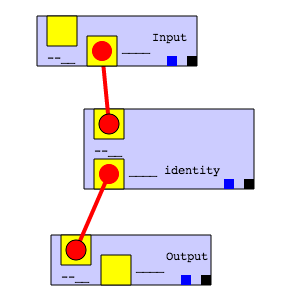
\includegraphics[width=0.35\textwidth]{./images/ref} \\
\caption{Reference to saved items. The definition of \code{identity} is shown in Figure~\ref{fig:defbody}.}\label{fig:ref}
\end{figure}

\subsubsection{Description of the GUI}
Figure~\ref{fig:gui} shows the basic layout of the GUI.
\begin{figure}[h]
\center
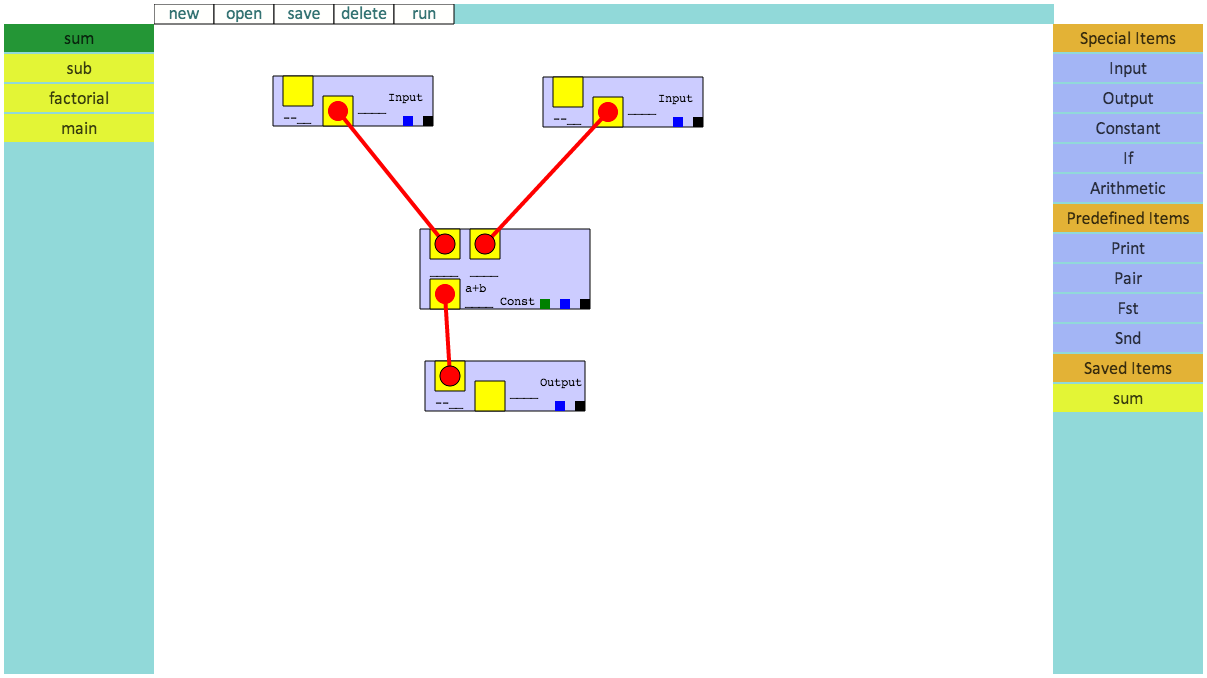
\includegraphics[width=.95\textwidth]{./images/gui.png} \\
\caption{The basic layout of the GUI.}\label{fig:gui}
\end{figure}
The top row of the GUI is the menu, which provides basic functionality of manipulating user-defined definitions. Users are able to create new function definitions, open existing function definitions, delete unwanted definitions and save definitions as black-box functions. The left side bar shows a list of user-defined functions, while on the right side are the special definitions and predefined functions. If a user-defined function is saved, it is also listed in the saved items and is ready for to be used in other definitions. The central region shows the function currently being constructed, which displays all the member nodes of current definition. The member nodes are references to either special definitions or functions (both predefined and user-defined ones). Each node has input anchors and one output anchor, except for nodes referring to special definitions such as input definition or constant definition.

The central region only displays the function currently being defined, and users can switch between different function definitions using the left side bar. Items listed on the right side bar can be added to current definition as member nodes. Nodes on current definition can also be deleted if no longer needed.

The member nodes in a definition is connected by links between output anchors and input anchors. A link represents using the output from the one node as the input for the other node. A node can have output links to multiple nodes, and a node having multiple inputs can link to output anchors of different nodes.

Special nodes are added to represent special definitions. The node representing \code{input} doesn't have any input anchor, while the node for \code{output} can have only one input anchor. \code{constant} node has a field for inputting the content of the constant, while \code{recursion} node has the same number of inputs as current definition. The \code{arithmetic} node is able to adjust its size and number of inputs depending on the input expression.

\subsection{Type-checking and Evaluation}



\section{Implementation Details}
\subsection{GUI}
The GUI is implemented in Javascript using the Kinetic Library\footnote{http://kineticjs.com/}. The implementation of the GUI has two major components: the basic GUI and the nodes. The basic GUI is the platform that support the definition-level operations, e.g. creation and deletion of function definitions and modification of the body the definitions. The nodes are the basic elements that represent elementary functional units of a program, which are essentially references to existing definitions and appear as rectangular boxes in a definition body. 

The graphical elements in the GUI are organized in a hierarchical structure. The top level is a stage, which is the container for the layers representing each individual user-defined function. Each user defined function is associated with a layer, and all its member nodes reside in that layer. Definition level user interactions correspond to operations on the layers: switching between different definitions is equivalent to switching between layers, adding or removing functional units to a definition is represented by adding or removing nodes to a layer, and deleting a definition is accomplished by deleting a layer in the GUI.

The nodes used to represent single functional units are in the lowest level in the GUI hierarchy. They are represented by a group of graphical elements: input anchors, output anchor, bounding box and labels. Figure~\ref{fig:node} show a typical node structure. On the top are a set of input anchors, while the circle on the bottom of the bounding box is the output anchor. The labels are used for type information as well as showing the name of the referred definition. The blue square on the bottom-right corner is a short-cut for disconnecting all input/output links of the node, and the black one is used for deleting the node.
\begin{figure}[h]
\center
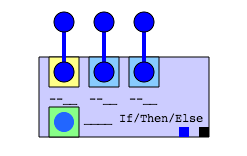
\includegraphics[width=0.3\textwidth]{./images/node} \\
\caption{A typical node.}\label{fig:node}
\end{figure}

Each node stores the definitions it is referring to as well as the definition it is in. The nodes also maintain a list of inputs and outputs by tracking the nodes they are connected to.

\subsection{Type-checking}
\begin{mathpar}
  \inferrule[Refl]{
    E(x) = \forall\alpha_1\dots\alpha_n.\tau
    \and
    Dom(\rho) \subseteq \{\alpha_1\dots\alpha_n\}
  }{
    E \vdash x : \rho(\tau)
  }
  \\
  \inferrule[Number]{}{E \vdash n : \type{number}}
  \and
  \inferrule[Boolean]{}{E \vdash b : \type{bool}}
  \and
  \inferrule[String]{}{E \vdash s : \type{string}}
  \\
  \inferrule[Node]{
    E \vdash f : (\tau) -> \tau_r
    \and
    E \vdash a_n : \tau_n
  }{
    E \vdash \code{node} n (a_1, \dots, a_n) : \tau_r
  }
  \\
  \inferrule[Function Definition]{
    E \vdash f : (\tau) -> \tau_r
    \and
    E \vdash a_n : \tau_n
  }{
    E \vdash \code{fundef} f(a_1, \dots, a_n) : \tau_r
  }
\end{mathpar}

\subsection{Evaluation}
Our evaluation strategy attempts to be pure, strict, and eager in all
cases where it makes sense. Nodes are evaluated only once, with
repeated evaluation available only through recursion. All arguments
are evaluated before the node itself is evaluated (with the important
exception of \code{if} expression). Furthermore, nodes which are not
required via this approach are {\em not} evaluated. This means
evaluation is most intuitively understood as a depth-first search for
a solution from the output node.

As mentioned above, \code{if} expressions do not respect the eager
evaluation of arguments. The conditional is evaluated first and then
only the branch selected is searched. This can be used with the
\type{world} type to implement flow control and with other types to
implement base cases for recursion.

\section{Conclusion}
We designed and implemented a 2D programming language in this project. 

\end{document}
